\documentclass{scrartcl}
\usepackage[margin=3cm]{geometry}
\usepackage{amsmath}
\usepackage{amssymb}
\usepackage{amsthm}
\usepackage{blindtext}
\usepackage{datetime}
\usepackage{fontspec}
\usepackage{graphicx}
\usepackage{kotex}
\usepackage{mathrsfs}
\usepackage{mathtools}
\usepackage{pgf,tikz,pgfplots}
\usepackage{float}

\pgfplotsset{compat=1.15}
\usetikzlibrary{arrows}

\newcommand\Overline[2][0.8pt]{%
  \begin{tikzpicture}[baseline=(a.base)]
    \node[inner xsep=0pt,inner ysep=1.5pt] (a) {$#2$};
    \draw[line width= #1] (a.north west) -- (a.north east);
  \end{tikzpicture}
}
\newtheorem{theorem}{Theorem}

\setmainhangulfont{Noto Serif CJK KR}[
  UprightFont=* Light, BoldFont=* Bold,
  Script=Hangul, Language=Korean, AutoFakeSlant,
]
\setsanshangulfont{Noto Sans CJK KR}[
  UprightFont=* DemiLight, BoldFont=* Medium,
  Script=Hangul, Language=Korean
]
\setmathhangulfont{Noto Sans CJK KR}[
  SizeFeatures={
    {Size=-6,  Font=* Medium},
    {Size=6-9, Font=*},
    {Size=9-,  Font=* DemiLight},
  },
  Script=Hangul, Language=Korean
]
\title{MATH230: Homework 13 (due Dec. 4)}
\author{손량(20220323)}
\date{Last compiled on: \today, \currenttime}

\newcommand{\un}[1]{\ensuremath{\ \mathrm{#1}}}
\newcommand{\imag}{\operatorname{Im}}
\newcommand{\real}{\operatorname{Re}}
\newcommand{\Log}{\operatorname{Log}}
\newcommand{\Arg}{\operatorname{Arg}}
\DeclareMathOperator*{\Res}{Res}

\begin{document}
\maketitle

\section{Chapter 10 \#4}
Let's state the null hypothesis \(H_0\) as \(p = 0.6\), and the alternative
hypothesis \(H_1\) as \(p < 0.6\).

\subsection{Solution for (a)}
Let \(X\) be the number of orders that arrived late. Then, \(X\) follows
\(b(10; p)\). The problem statement suggests that the \(H_0\) is rejected if
\(X \le 3\). We can write the type I error probability \(\alpha(p)\) as
\begin{align*}
  \alpha(p)
  = \sum^3_{x = 0} {10 \choose x} p^x (1 - p)^{10 - x}
\end{align*}
Then we obtain \(\alpha(0.6) = 0.0547618816\).

\subsection{Solution for (b)}
\(H_0\) is accepted if \(X > 3\). We can write the type II error probability
\(\beta(p)\) as
\begin{align*}
  \beta(p)
  = \sum^{10}_{x = 4} {10 \choose x} p^x (1 - p)^{10 - x}
\end{align*}
Then we obtain \(\beta(0.3) = 0.3503892816, \beta(0.4) = 0.6177193984,
\beta(0.5) = 0.828125\).

\section{Chapter 10 \#15}
Let's state the null hypothesis \(H_0\) as \(\mu = 200\), and the alternative
hypothesis \(H_1\) as \(\mu \not = 200\).

\subsection{Solution for (a)}
Let \(\bar{X}\) be a sample mean of nine samples. Then \(H_0\) is rejected if
\(|\bar{X} - 200| \ge 9\). Let \(Z = \sqrt{9}(\bar{X} - \mu) / 15\), then
\(Z \sim N(0, 1)\). Thus, \(H_0\) is rejected if \(|Z| \ge 9/5\) and the
probability we are looking for is \(P(|Z| \ge 9/5) = 0.07186064\).

\subsection{Solution for (b)}
When \(\mu = 215\), then \(H_0\) is accepted if \(|\bar{X} - 200| < 9\), which
is equivalent to \(-24/5 < Z < -6/5\). The probability we are looking for is
\(P(-24/5 < Z < -6/5) = 0.1150689\).

\section{Chapter 10 \#18}
For given value of \(\mu\), \(H_0\) is accepted if \(|\bar{X} - \mu| < 0\),
which is equivalent to
\begin{align*}
  \frac{\mu - 209}{5}
  < Z
  < \frac{\mu - 191}{5}
\end{align*}
Now, the probabilities of failing to reject \(H_0\) for given values of \(\mu\)
can be calculated with the formula above. They are 0.08075637, 0.27423977,
0.57892278, 0.83668356, 0.92813936, 0.83668356, 0.57892278, 0.27423977, and
0.08075637 respectively. The OC curve can be plotted as below:
\begin{figure}[H]
  \centering
  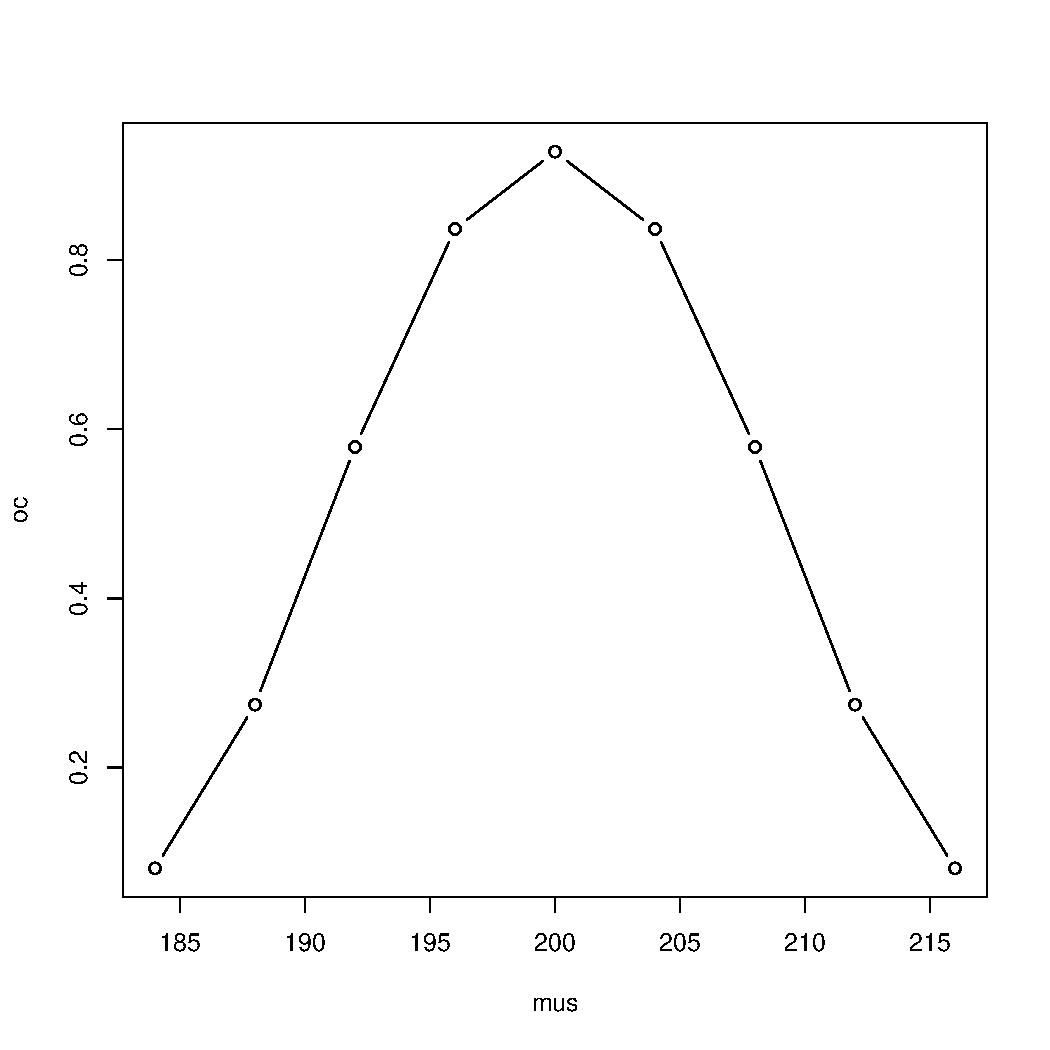
\includegraphics[width=0.7\linewidth]{ocplot.pdf}
\end{figure}

\section{Chapter 10 \#20}
Let \(n = 49, \bar{x} = 970, \sigma = 70, \alpha = 0.05, \mu_0 = 1000\) and the
null hypothesis \(H_0\) and the alternative hypothesis \(H_1\) as \(\mu =
\mu_0, \mu < \mu_0\), respectively. We can write
\begin{align*}
  \frac{\sqrt{n} (\bar{x} - \mu_0)}{\sigma}
  = -3
  < -z_\alpha
  = -1.644854
\end{align*}
so we can reject \(H_0\) at 0.05 level of significance.

\section{Chapter 10 \#24}
Let \(n = 54, \bar{x} = 7.2, \sigma = 1.4, \mu_0 = 8.4\), and the null
hypothesis \(H_0\) and the alternative hypothesis \(H_1\) as \(\mu = \mu_0\)
and \(\mu \not = \mu_0\), respectively. We can write the \(P\)-value as
\begin{align*}
  P
  = 2P \left( Z
    > \left| \frac{\sqrt{n} (\bar{x} - \mu_0)}{\sigma} \right| \right)
    = 3.001757 \times 10^{-10} < 0.05
\end{align*}
where \(Z \sim N(0, 1)\). Thus, we can reject \(H_0\) and conclude that the
average distance changed.

\end{document}
% vim: textwidth=79
